\chapter{Nitric Oxide Reduction in \Nm{}}

Modelling nitric oxide reduction involves adding nitric oxide whilst cultures are respiring aerobically. The conditions are the same as for oxygen reduction, except that nitric oxide solution is added to a concentration of $\mathrm{\approx 5\mu M}$ and the culture then left to respire nitric oxide.

In the model, Equations (2, 7 \& 9) are now involved, as the nitric oxide reductase NorB is being used in addition to the requirement to model the chemical inhibition of $\mathrm{cbb}_3$ by nitric oxide. The parameter posterior probability distributions generated from the Monte-Carlo runs from the oxygen reduction dataset were used as prior probability distributions for this next dataset. The unknown parameters (those not included in the previous dataset) were set to sensible non-zero values which would allow them to burn-in and generate subsequent posterior distributions.
The datasets used for this section of the model describe the effect on oxygen reduction as nitric oxide is introduced to a system that is only partially primed for microaerobic respiration. There will be a small amount of NorB (the nitric oxide reductase) present to remove and nitric oxide that is present. The $\mathit{nsrR}^-$ mutant, which expresses NorB in an essentially constitutive manner was not effective in generating a usable dataset as it removed any NO almost instantaneously resulting in an almost featureless dataset (data not shown).

The dataset and final solved output from the Monte-Carlo run are show in figure \ref{fig:nosim}. This is a more complex dataset than for oxygen respiration. Initially the oxygen reduction is carried out in exactly the same manner as the previous dataset, which is able to be modelled with the parameters selected from the prior distributions. Upon addition of nitric oxide, oxygen respiration slows and almost stops as a result of competition for electrons between $\mathrm{cbb}_3$ and NorB, and the direct chemical inhibition of $\mathrm{cbb}_3$ by NO. Nitric oxide starts being removed as a combination of simple diffusion (although this rate will be low) and reduction via NorB. Once the NO has been removed from the system oxygen reduction resumes at almost the same rate as before and still has the same high affinity feature as the previous dataset. The closeness of fit of the solved parameter set to the experimental data shows that the model has been able to accommodate a parameter set from the prior distributions that is able to accommodate all these features, and will still be able to model simple oxygen reduction.

\begin{figure}[ht!]
 \centering
 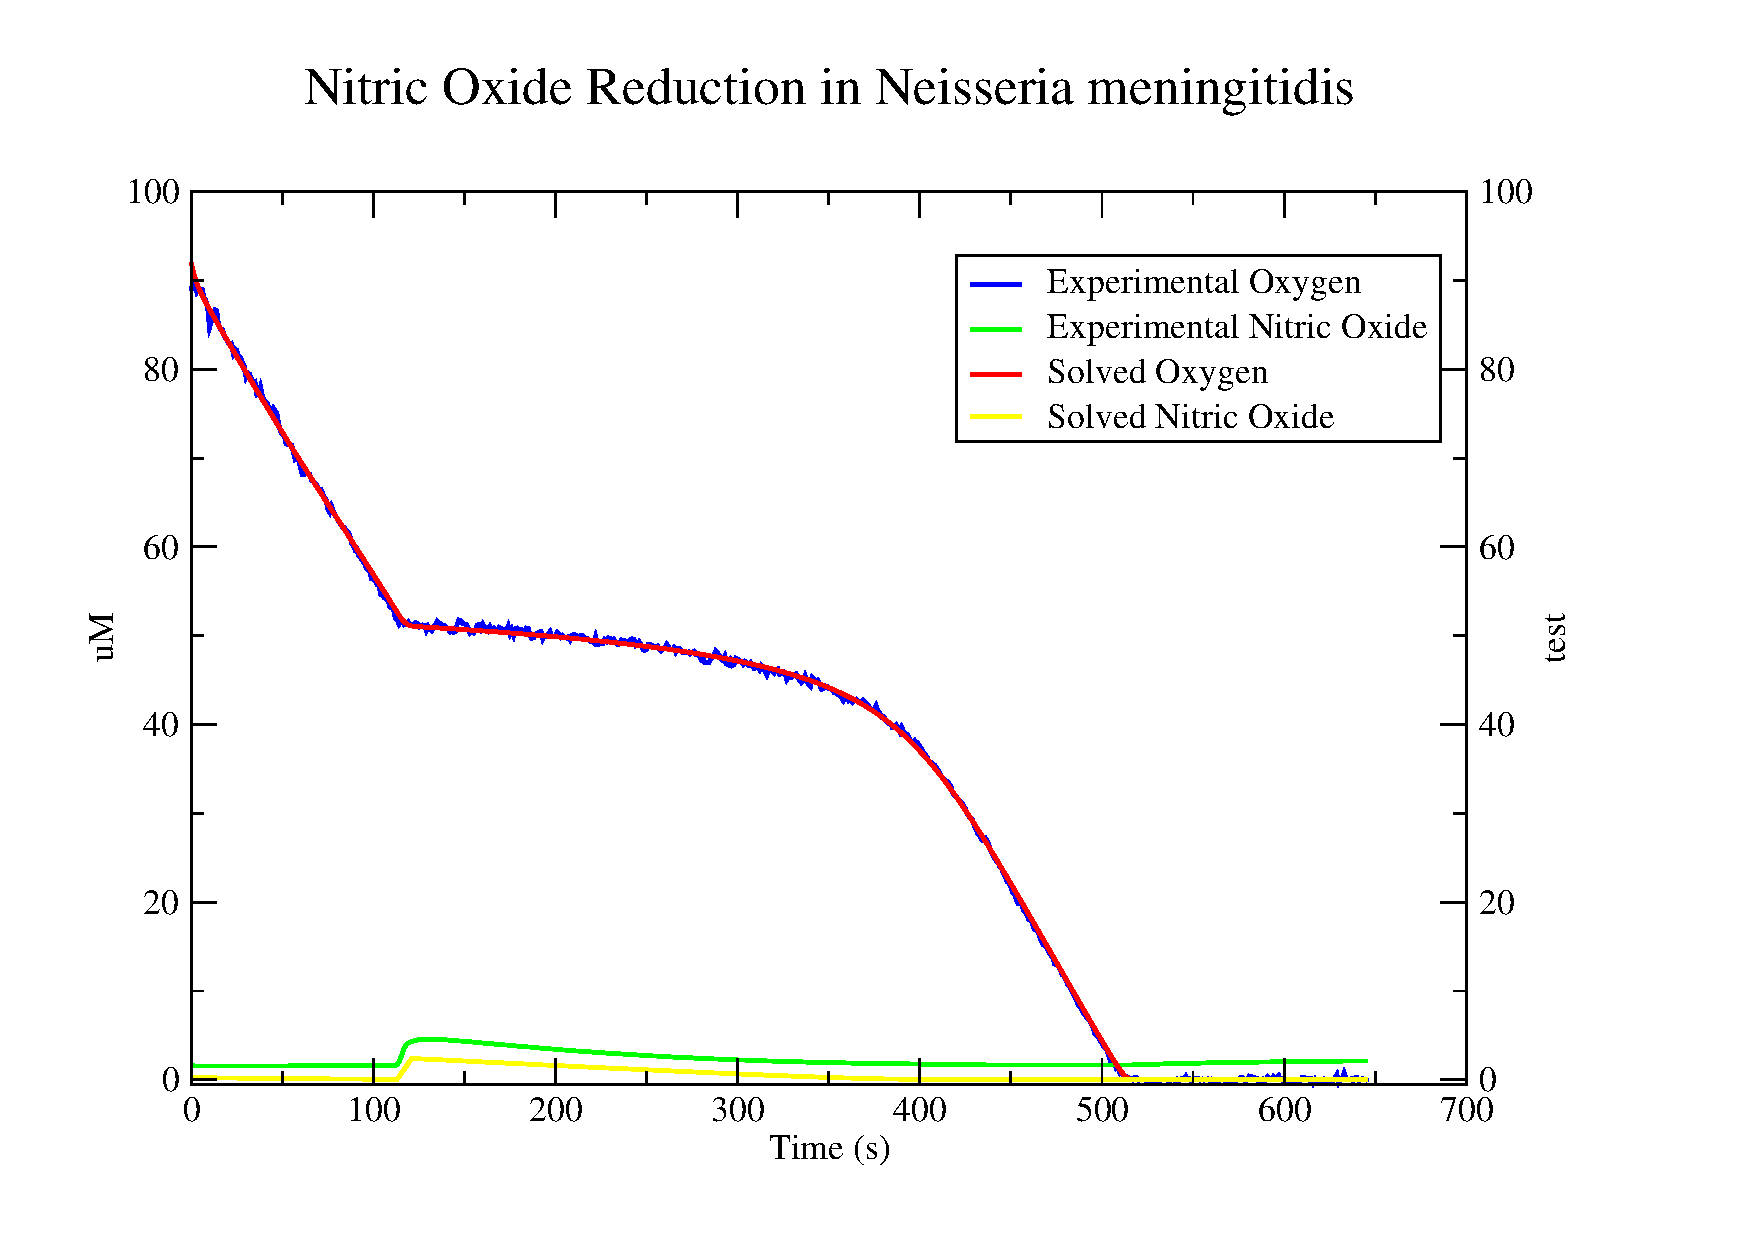
\includegraphics[width=14cm]{./06-noreduction/data/nosim.pdf}
 % nosim.eps: 0x0 pixel, 300dpi, 0.00x0.00 cm, bb=0 0 794 595
 \caption[{Nitric Oxide Reduction in \textit{Neisseria meningitidis}.}]{{\bf Nitric Oxide Reduction in \textit{Neisseria meningitidis}.} This dataset shows the effect on rate of oxygen reduction as nitric oxide is introduced to the system. The solved output, using prior probabilities from the oxygen reduction dataset show an almost perfect match to the features of the experimental dataset. The solved oxygen concentrations match the experimental dataset so closely as to be almost invisible.}
 \label{fig:nosim}
\end{figure}

\section{Aerobic Nitric Oxide Reduction}
\subsection{Introduction}
\subsection{Results}
\subsection{Discussion}
\section{Microaerobic Nitric Oxide Reduction}
\subsection{Introduction}
\subsection{Results}
\subsection{Discussion}
\section{Aerobic Nitric Oxide Reduction in \textit{nsrR$^\textrm{-}$} mutant}
\subsection{Introduction}
\subsection{Results}
\subsection{Discussion}